\chapter{Comparaison GCM - CCM - OCB}

Lors de nos recherches nous avons constaté que les algorithmes fournissant à la foi la confidentialité, l'authenticité et l'intégrité sont: GCM, CCM, OCB, CWC, EAX et APM.

Mais paris eux seulement trois sortent du lot GCM, OCB et CCM. C'est pourquoi nous avons décidé d'écarter les autres algorithmes et de seulement comparer ces trois.

\section{CCM}

Comme son nom le suggère le mode CCM combine le mode CTR et le mode CBC-MAC. C'est deux modes "primitfs" sont combinés pour authentifier les données puis les encrypter. CBC-MAC permet dans un premier temps d'obtenir un tag d'authentification du message clair. Puis le message et le tag sont chiffrés en utilisant le mode CTR.



L'une vecteur d'initialisation (IV) doit est être choisi avec précaution car il ne doit jamais être utilisé plus d'un fois par clef. En effet le mode CCM est un dérivé du mode CTR.



Une idée essentielle est que la même clé de cryptage peut être utilisé à la fois pour l'authentification et l'encryptage, à condition que les valeurs de comptage utilisées dans le cryptage ne rentrent pas en collision avec le vecteur d'initialisation (VI) utilisé pour l'authentification.


\begin{figure}[!h]
  \centering
  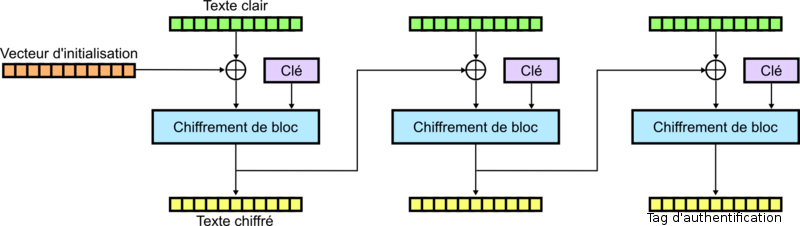
\includegraphics[width=\textwidth]{fonctionnement-CBC_MAC}
  \caption{Création du tag d'authentification avec CBC-MAC}
  \label{Création du tag d'authentification avec CBC-MAC}
\end{figure}

\begin{figure}[!h]
  \centering
  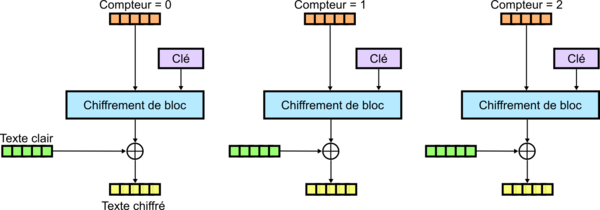
\includegraphics[width=\textwidth]{fonctionnement-CTR}
  \caption{Chiffrement du tag et du message avec CTR}
  \label{Chiffrement du tag et du message avec CTR}
\end{figure}

\newpage


\section{OCB}
Le mode OCB est lui aussi conçu pour fournir à la fois l'authentification et la confidentialité. OCB (Offset CodeBook) est basé sur le mode ECB avec l'utilisation d'un vecteur d'initialisation. Pour l'authentification il faut d'abord effectuer un checksum du message clair, ce checksum est ensuite encrypter comme un block du message clair. 

\begin{figure}[!h]
  \centering
  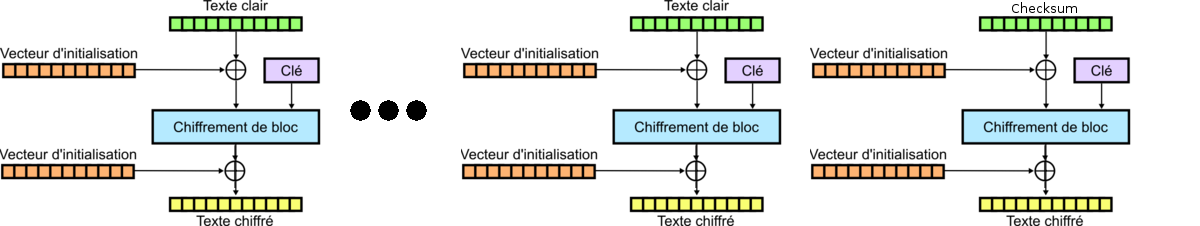
\includegraphics[width=\textwidth]{fonctionnement-OCB}
  \caption{Fonctionnement du mode OCB}
  \label{Fonctionnement du mode OCB}
\end{figure}



%%% Local Variables: 
%%% mode: latex
%%% TeX-master: "rapport_de_base"
%%% End: 
